\documentclass{article}

\usepackage{amsmath}
\usepackage[T1]{fontenc}
\usepackage[margin=2.5cm]{geometry}
\usepackage{comment}
\usepackage{graphicx}
\usepackage{float}


\begin{document}
\section{Introduction}
\subsection{The importance of aerodynamic studies}
At the beginning of writing of this appendix, it is valuable to emphasize the importance of 
aerodynamic studies in case of designing the rocket.  Not only do they decrease significantly 
the mass of the rocket but also they take a huge part in optimization of length and usage of 
materials, which are beneficial to our not so enormous budget. Apart from that, they increase 
the safety of the rocket in regards to testing its stability. Hence, by preforming these studies, 
you are capable of determining how the whole structure would behave before launching, which is 
necessary bearing in mind that it is not often that you get to test rocket models. This study 
was mainly based on “The Modern Exterior Ballistic” written by Robert L. McCoy.

\subsection{The problem of aerodynamic drag}
Rockets have several aerodynamics characteristics that are worth attention in order to 
estimate the performance after launch. However, in the event of designing non-controlling 
aerodynamically rockets such as ours, the most crucial factor is aerodynamic drag coefficient. 
Thanks to this variable it is possible to compare different configurations of the rocket so as to be able 
to choose the most lightest one. Although, R6 rocket doesn't exceed 1 Mach, drag coefficient 
may slightly vary depending on velocity of the rocket. This variable was calculated 
using following formula:
\begin{equation}
    F_d = \frac{1}{2} \rho v^2 C_d A \quad \equiv \quad C_d = \frac{2F_d}{\rho v^2 A}
\end{equation}
Where: $F_d$ - drag force gained from aerodynamic simulations, $C_d$ - drag coefficient, 
$\rho$ air density, v- velocity of the rocket, A - projectile reference area.\\\\


\begin{comment}
\subsection{Methodology of the present work}
For simulations we choose two programs to compare the results. The first one is 
Solidworks Flow Simulation, in which we also prepared models for simulations. 
The second one is Ansys Fluent.\\\\
First we prepared the models in Solidworks and from there we exported them to 
.step (214) file format to import them to Ansys. In Ansys we used Fluent with
Meshing to prepare the mesh and then we run the simulations. Solidworks Flow Simulation
was also used to prepare the mesh and run the simulations, which we later compared with
Ansys Fluent results.\\\\
All models were tested using Parametric studies/sets for 9 different velocities 
from 0.1 to 1.0. The resulting graphs of drag coefficient vs mach number were 
compared and analyzed.
\end{comment}

\subsection{Methodology of the present work}
For simulations, two programs were chosen to compare the results. The first program, 
Solidworks, was used for model preparation, reference simulations and parametric studies. The second 
program utilized was Ansys Fluent.\\\\
To determine optimal sweep angles and endcone angles, models of R6 Endcone and R6 NoEndcone were 
initially prepared in Solidworks. They were subsequently subjected to tests ranging from 0.1 to 1.0 
Mach, serving as reference points for future research. Following this, parametric studies were 
independently conducted for the endcone and fins. Each angle of the study underwent analysis at 
six different velocities. The results were subsequently analyzed and compared to ascertain the 
rocket's optimal configuration.\\\\
For simulations in Solidwors and in Ansys, adiabatic flow was assumed and friction forces were
neglected. Ansys solver calculated denisty changes using ideal gas equation.\\\\
Furthermore, the stability of the models was assessed using OpenRocket, accounting f
or stability changes arising from variations in endcone and fins angles.



\subsection{Tested models}
Various variations of the rocket were tested to ascertain the optimal configuration before 
finalizing its geometry. Firstly, the PrawieR5 rocket model, a modified version from the previous year's competition 
was examined. Subsequently, research was conducted to evaluate the impact of the endcone on 
aerodynamic parameters. This involved testing two models: R6 Endcone and R6 NoEndcone. Both models exhibited identical stability. Afterward, the endcone and fins optimalization
was contucted on R6 Endcone model.


\newpage
\section{Initial study}
The work was initiated with the remodeled R5, which had been prepared in Solidworks 
and featured an endcone, a modification in comparison to the original R5 model. Subsequent 
testing of the model was conducted using Solidworks Flow Simulation. However, this model 
was solely utilized for comparing the results of the older model with the new one. The 
results can be observed bellow.

\begin{figure}[H]
    \centering
    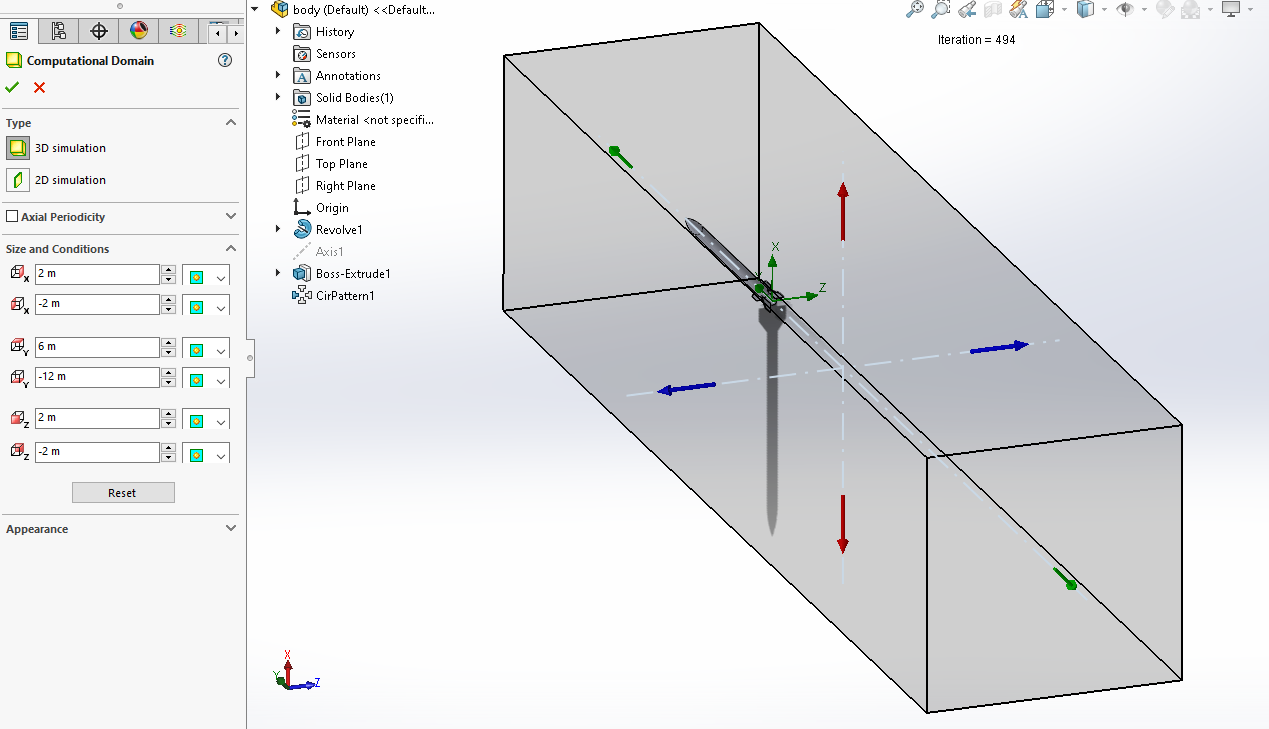
\includegraphics[width=\textwidth]{../data/PrawieR5-Solid/ComputationalDomain.png}
    \caption{CD graph for PrawieR5 model at Mach 0.6}
\end{figure}

\begin{figure}[H]
    \centering
    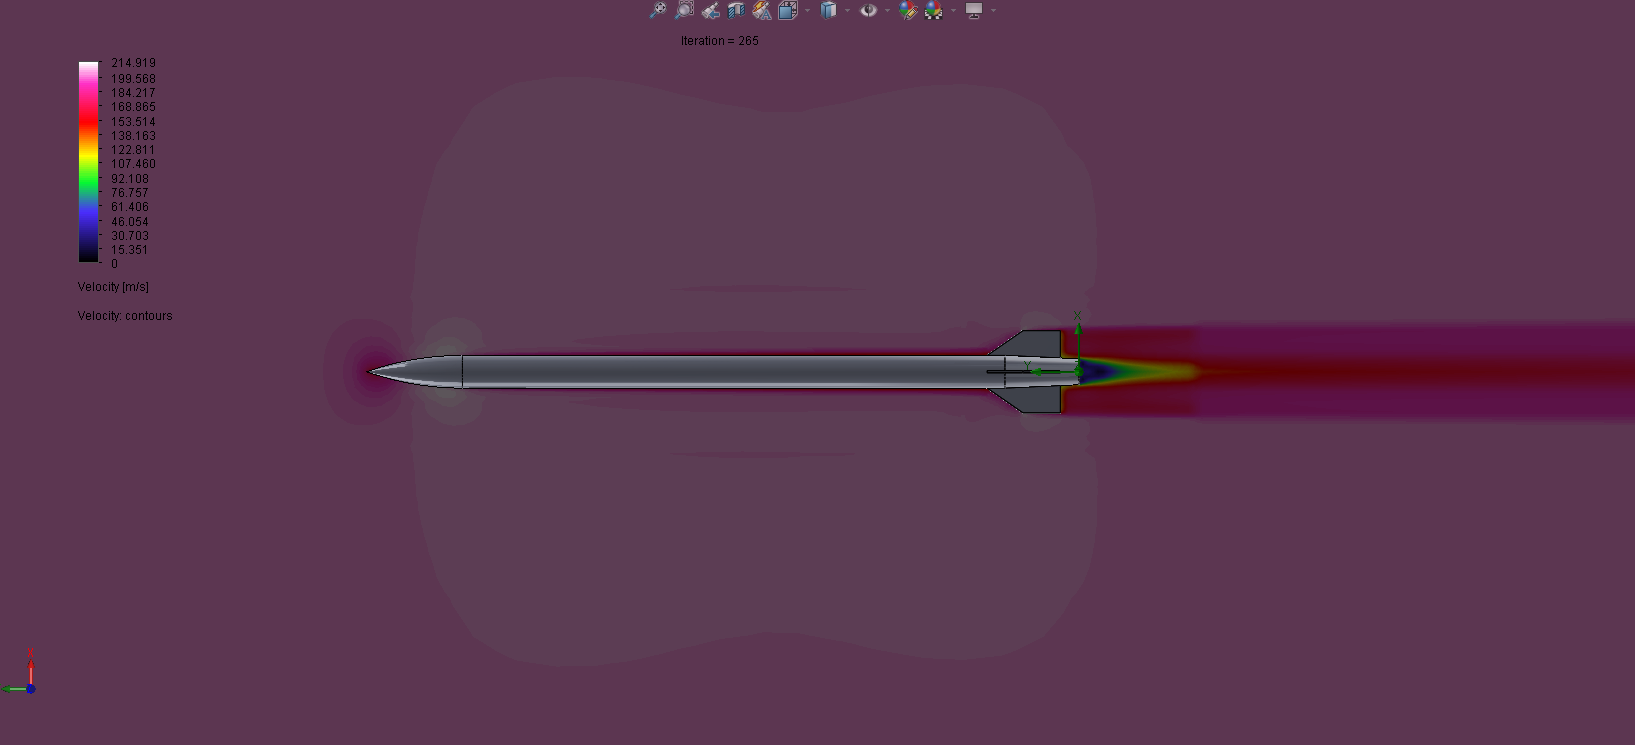
\includegraphics[width=\textwidth]{../data/PrawieR5-Solid/PrawieR5-TR-Velocity-Mach06.png}
    \caption{Velocity graph for PrawieR5 model at Mach 0.6}
\end{figure}




\section{Preliminary research of endcone effect in Solidworks}
\subsection{R6 Endcone}
\begin{figure}[H]
    \centering
    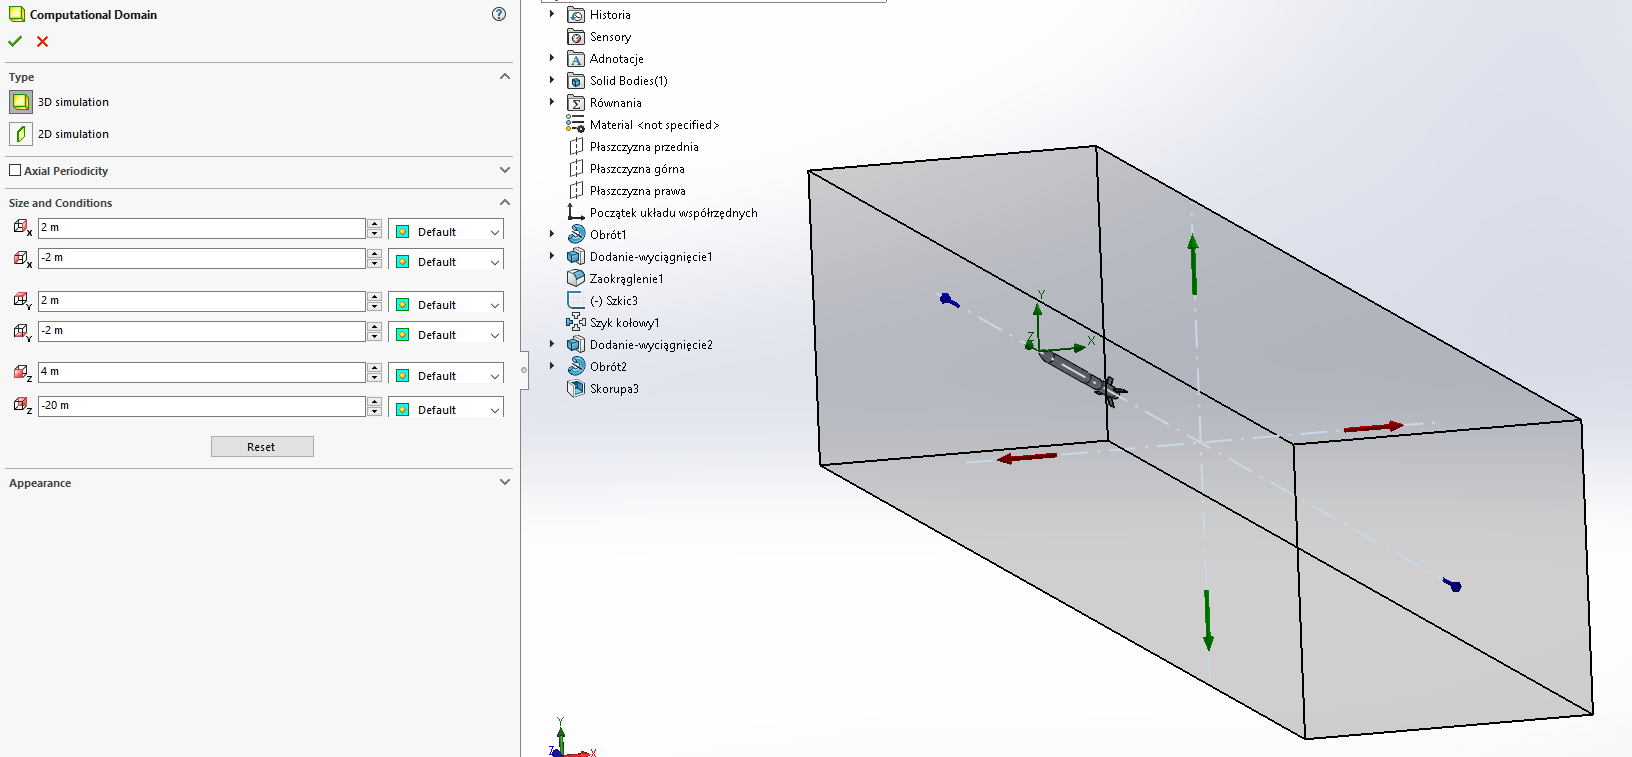
\includegraphics[width=\textwidth]{../data/R6-Endcone-Solid/domain.png}
    \caption{Computational domain for R6-Endcone model}
\end{figure}
\begin{figure}[H]
    \centering
    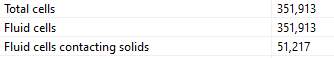
\includegraphics[width=0.6\textwidth]{../data/R6-Endcone-Solid/cells.png}
    \caption{Cell number for R6-Endcone model}
\end{figure}

\begin{figure}[H]
    \centering
    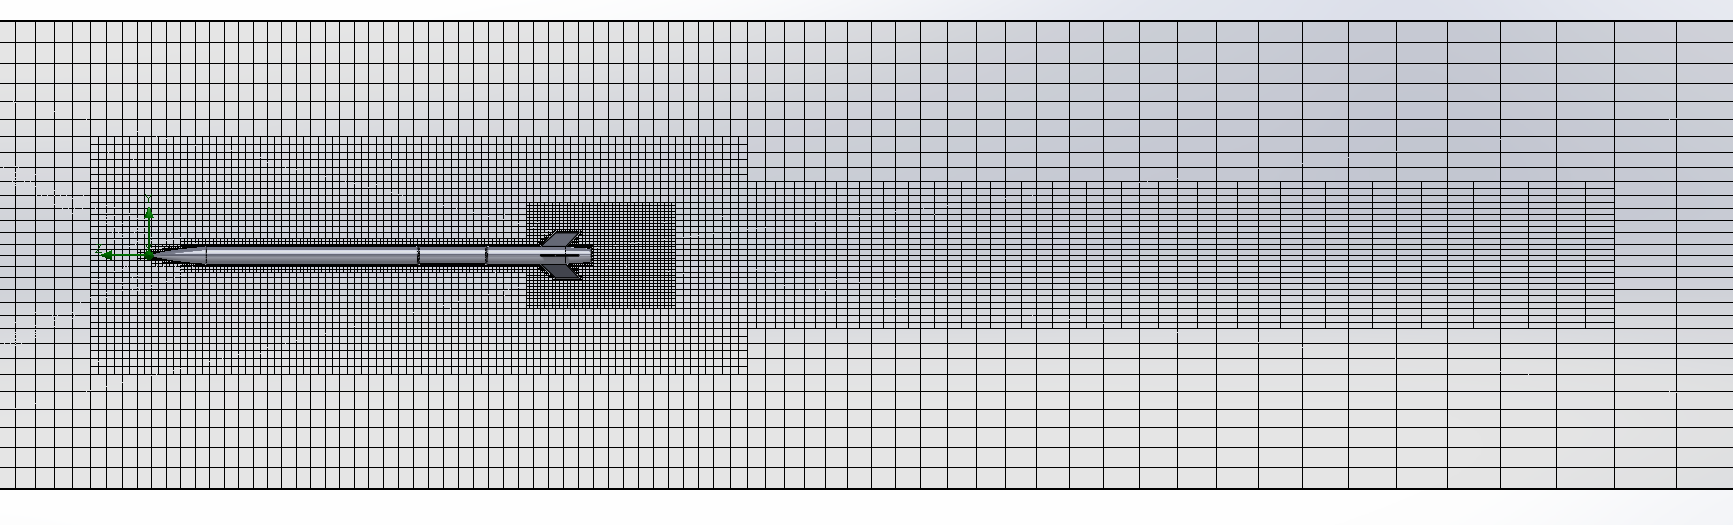
\includegraphics[width=\textwidth]{../data/R6-Endcone-Solid/mesh.png}
    \caption{Mesh for R6-Endcone model}
\end{figure}
\begin{figure}[H]
    \centering
    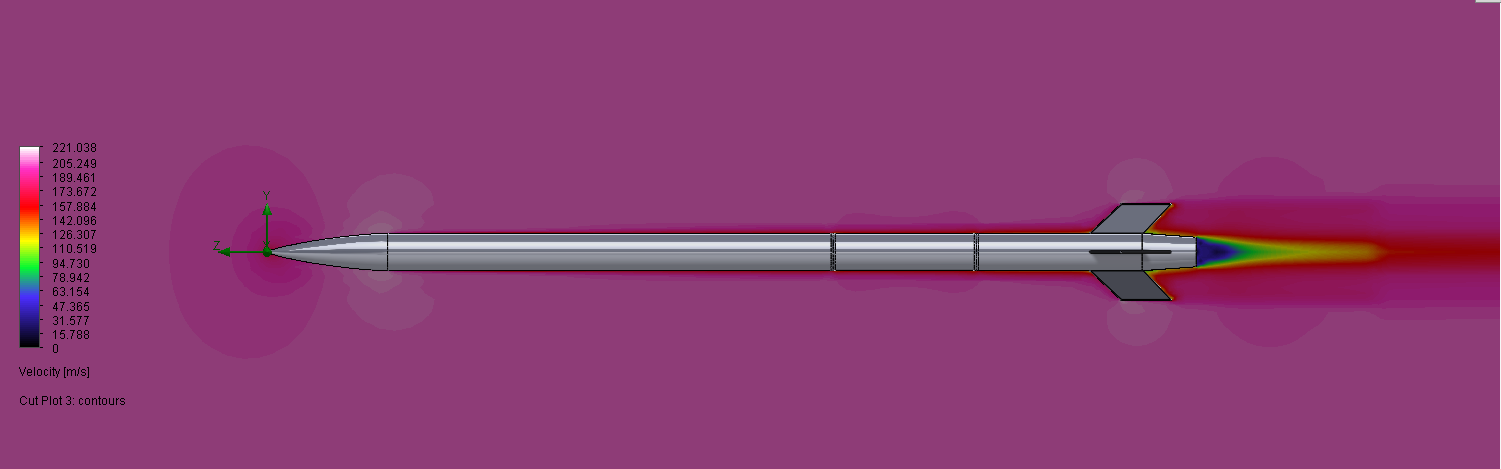
\includegraphics[width=\textwidth]{../data/R6-Endcone-Solid/speed.png}
    \caption{Velocity graph at 0.6 Mach for R6-Endcone model}
\end{figure}

\begin{figure}[H]
    \centering
    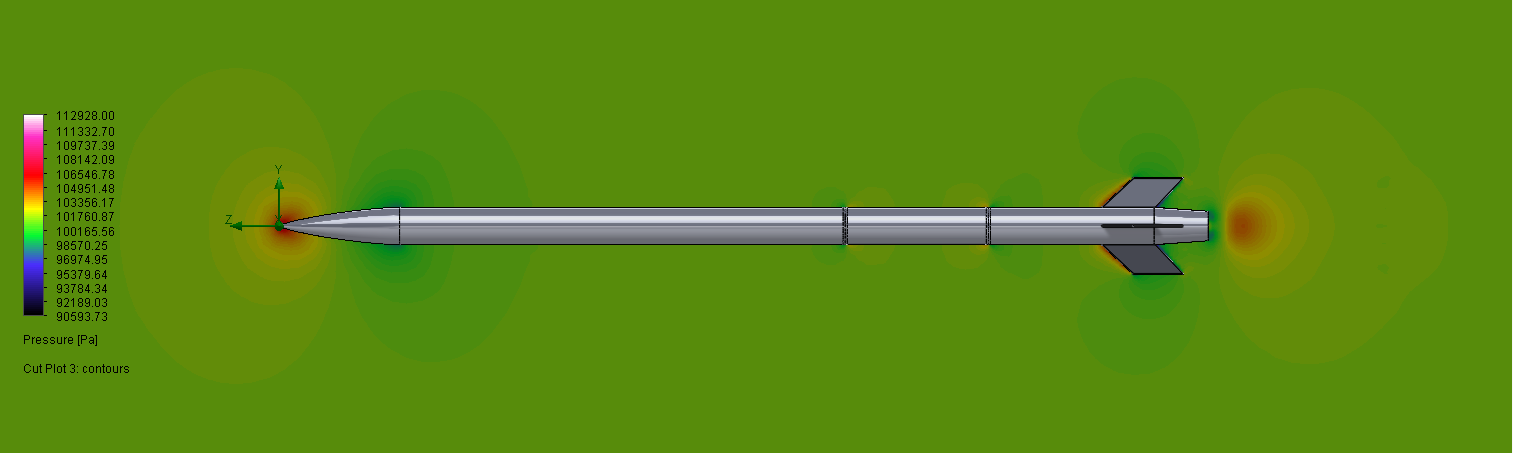
\includegraphics[width=\textwidth]{../data/R6-Endcone-Solid/pressure.png}
    \caption{Pressure graph at 0.6 Mach for R6-Endcone model}
\end{figure}

\subsection{R6 No Endcone}

\begin{figure}[H]
    \centering
    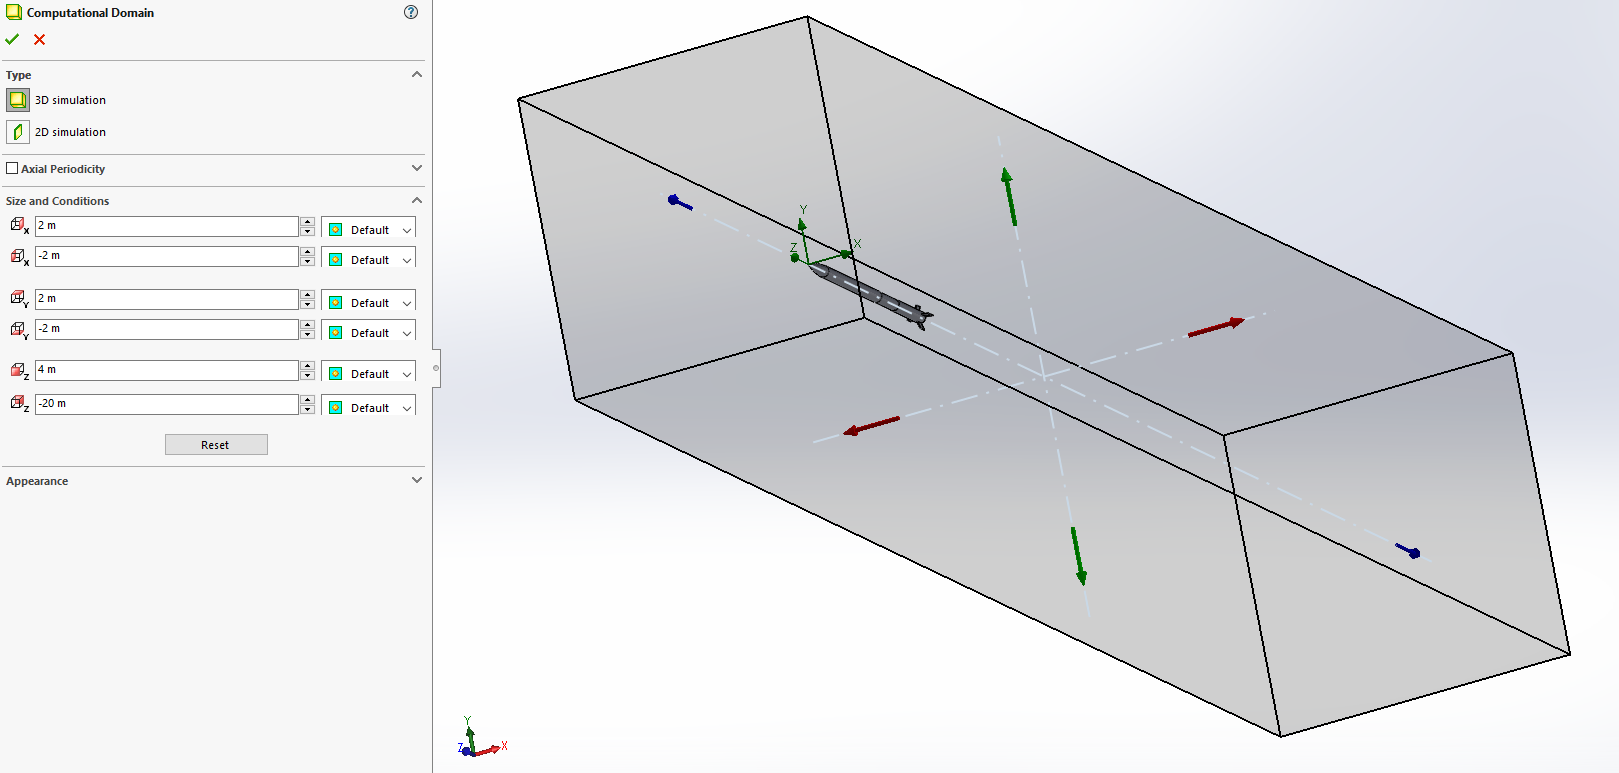
\includegraphics[width=\textwidth]{../data/R6-NoEndcone-Solid/domain.png}
    \caption{Computational domain for R6-NoEndcone model}
\end{figure}
\begin{figure}[H]
    \centering
    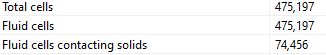
\includegraphics[width=0.6\textwidth]{../data/R6-NoEndcone-Solid/cells.png}
    \caption{Cell number for R6-NoEndcone model}
\end{figure}

\begin{figure}[H]
    \centering
    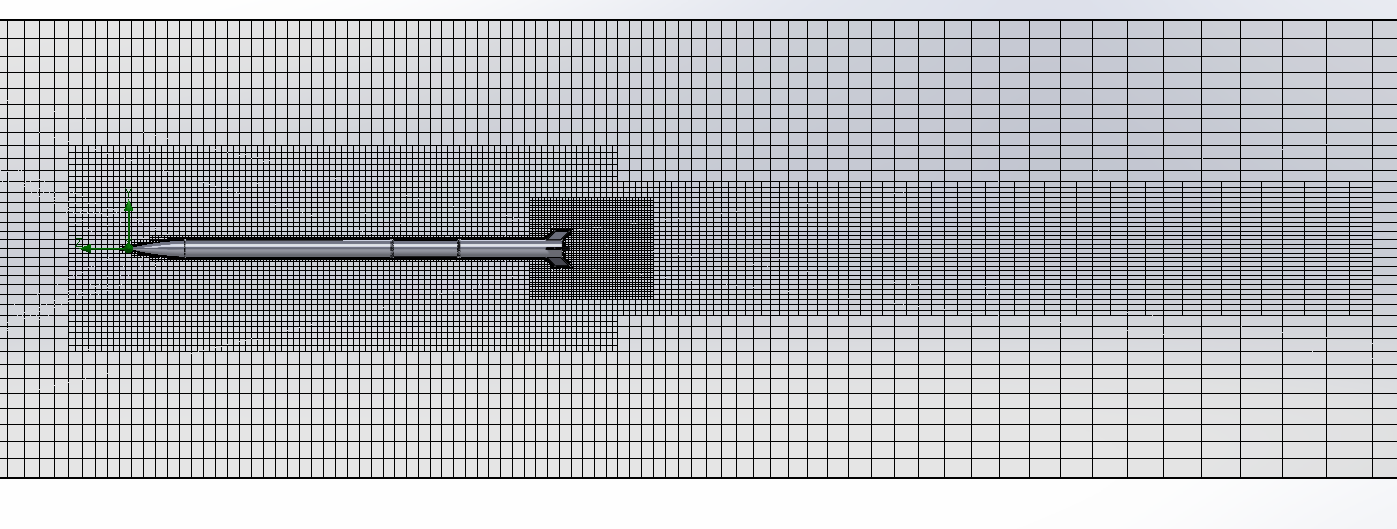
\includegraphics[width=\textwidth]{../data/R6-NoEndcone-Solid/mesh.png}
    \caption{Mesh for R6-NoEndcone model}
\end{figure}
\begin{figure}[H]
    \centering
    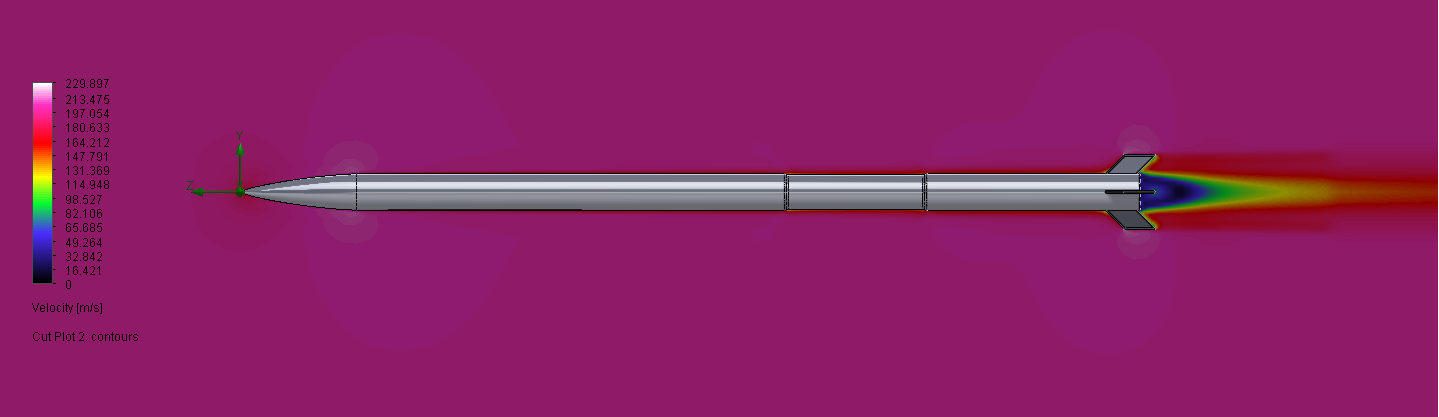
\includegraphics[width=\textwidth]{../data/R6-NoEndcone-Solid/speed.png}
    \caption{Velocity graph at 0.6 Mach for R6-NoEndcone    model}
\end{figure}

\begin{figure}[H]
    \centering
    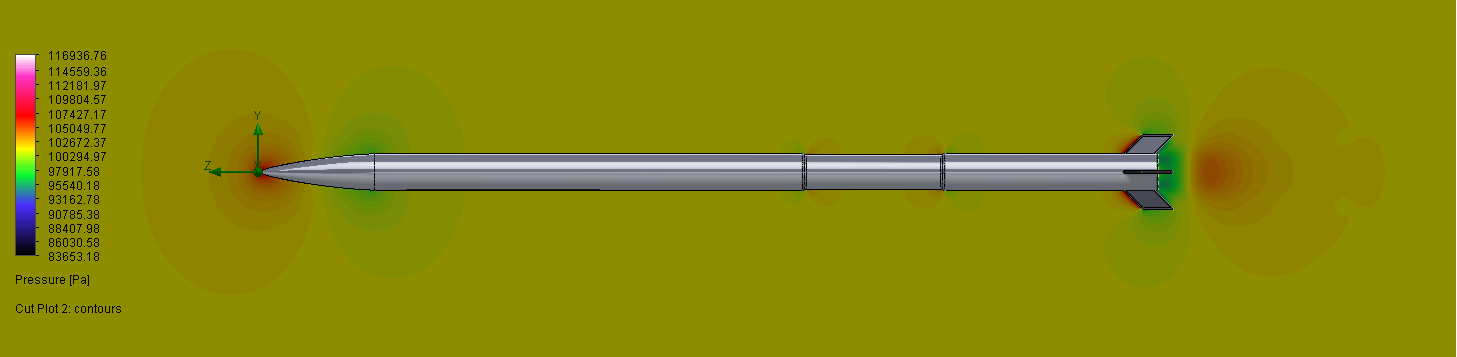
\includegraphics[width=\textwidth]{../data/R6-NoEndcone-Solid/konospeedoatode.png}
    \caption{Pressure graph at 0.6 Mach for R6-NoEndcone model}
\end{figure}



\section{Oplitmalization of the endcone in Solidworks}
\subsection{Range and goal of this study}
The goal of this study was to find a minimum of the average drag force function, depending on
the endcone angle, which was coupled to the lenght of the endcone. The range of the
study was from 3 to 15 degrees, with a step of 1 degree. For each angle, simulations were preformed for 
0.1 to 0.6 Mach, with a step of 0.1 Mach. In total 96 simulations were made, however it since 
lenghts of encone for angle values of 0 - 3 were too big, those where deleted from study.\\\\
Finding minimum of the average drag force function is crucial for the optimalization of the rocket
since that would allow to reduce the drag force acting on the rocket, which would result in
overall better performance of the rocket.\\\\
Function of drag coefficient for different Mach number depending on the endcone angle is also 
shown in the graph. It allows to determine the optimal angle for the endcone for specific
velocity and can be compared with existing literature.\\\\
Mesh and domain settings for following simulations are the same as in the preliminary research for
R6-Endcone model. Cell count changed slightly with the change of the endcone angle, but it was
negligible.

\subsection{Results}

\begin{figure}[H]
    \centering
    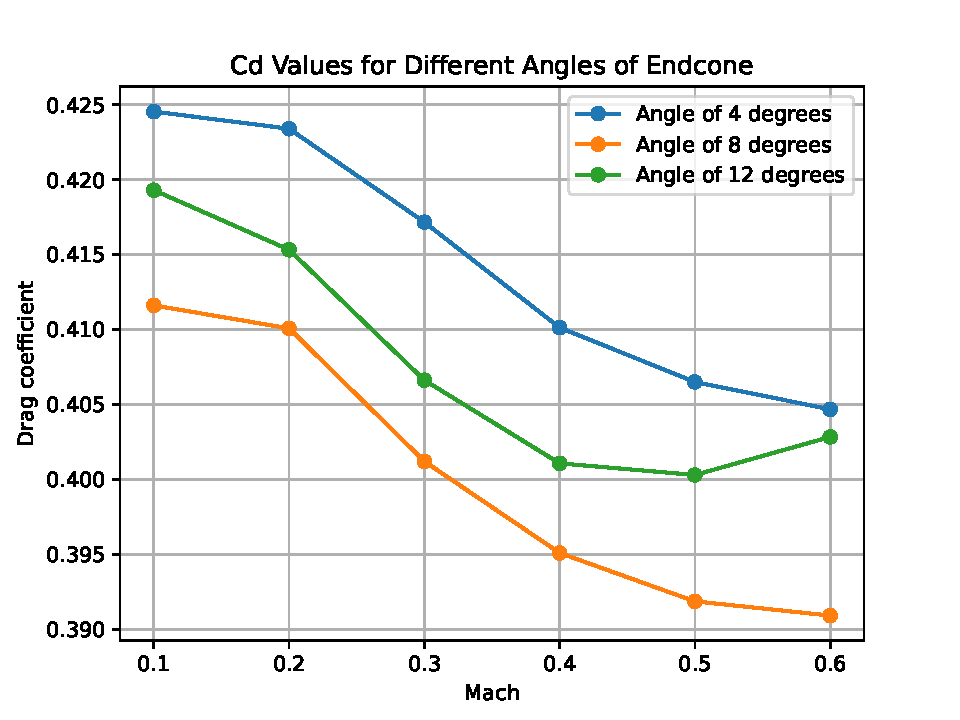
\includegraphics[width=0.9\textwidth]{../data/R6-Parametric-Endcone/ExampleCdGraphs.pdf}
    \caption{Example of CD graphs for different endcone angles}
\end{figure}

\begin{figure}[H]
    \centering
    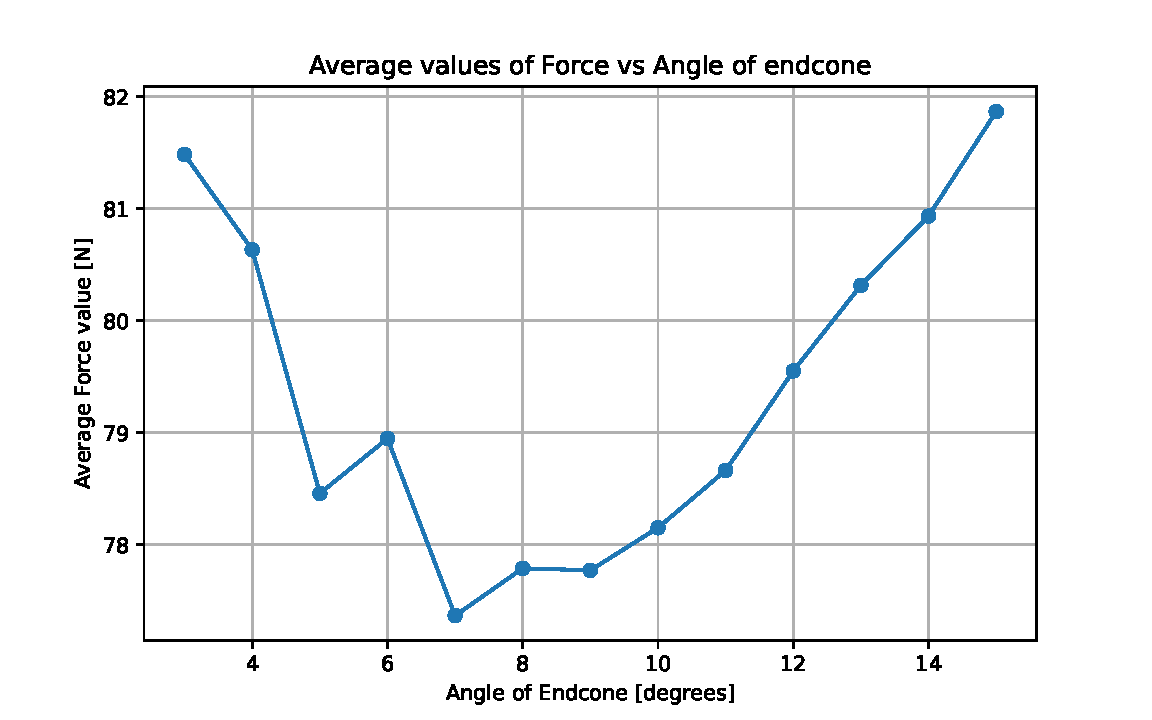
\includegraphics[width=\textwidth]{../data/R6-Parametric-Endcone/ForceVsAngle.pdf}
    \caption{Average Force vs Angle graph}
\end{figure}


\begin{figure}[H]
    \centering
    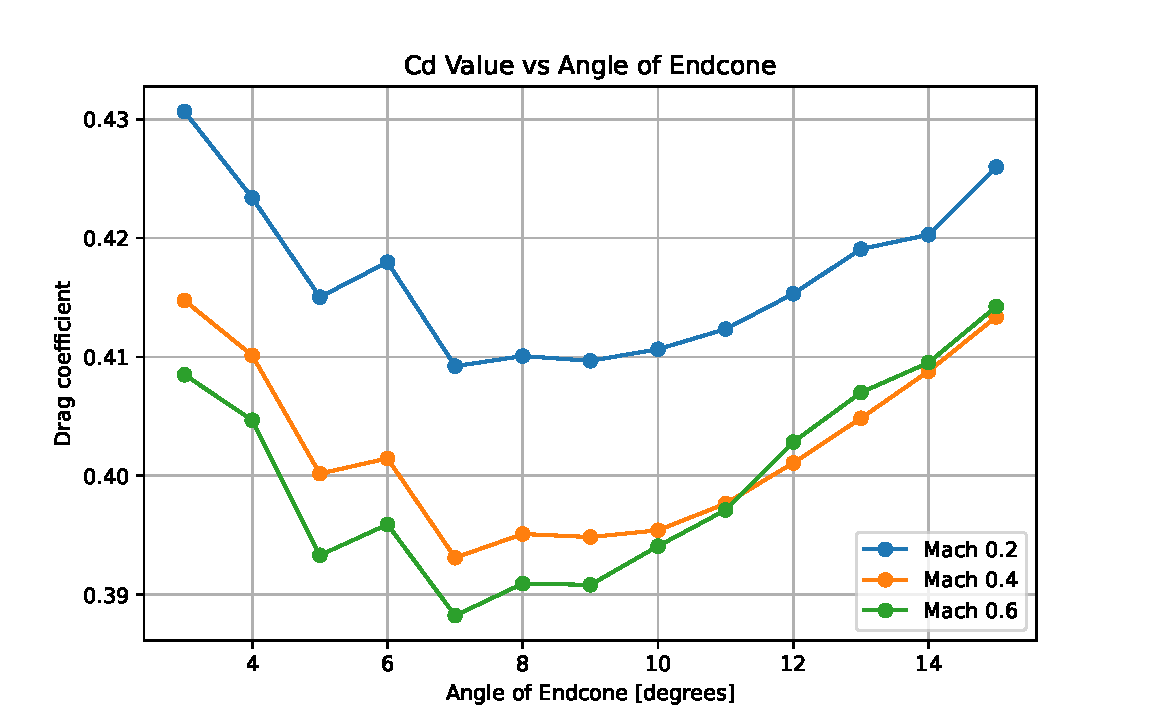
\includegraphics[width=0.9\textwidth]{../data/R6-Parametric-Endcone/CdVsAngle.pdf}
    \caption{Drag coefficient vs Angle graph}
\end{figure}



\newpage

\section{Optimalization of the fins in Solidworks}
\subsection{Range and goal of this study}
The goal of this study was to find the most optimal sweep angle of the fins for the R6 model. 
Only parameter was 90 degrees minus sweep angle, the lenght of top of fin, lenght of bottom of fin and height of 
fin were kept constant. The range of the study was from 30 to 90 degrees, with a step of 5 degree. 
For all sweep angle values, simulations were preformed for 0.1 to 0.6 Mach, with a step of 0.1 Mach.\\\\
Mesh and domain were kept the same as in prior simulations. Cell count changed slightly with the 
change of the sweep angle, similiar to the endcone study, it was negligible.\\\\
Endcone angle this time was kept at 4.29 degrees, since the physical model of it was already made.\\\\
One important note is that for the rest of this study, we will call the angle 90 degrees minus sweep 
angle just sweep angle.\\\\


\subsection{Results}
\begin{figure}[H]
    \centering
    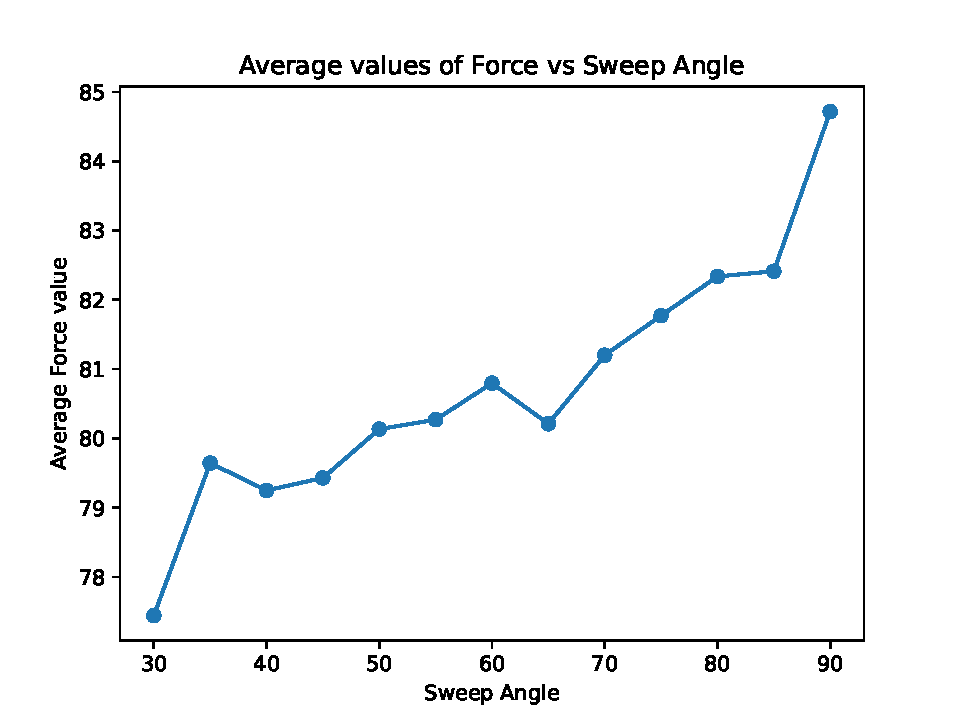
\includegraphics[width=1\textwidth]{../data/R6-Parametric-Fins/ForceVsSweepAngle.pdf}
    \caption{Average Force Value vs Sweep Angle}
    \label{fig:ForceVsSweepAngle}
\end{figure}

\begin{figure}[H]
    \centering
    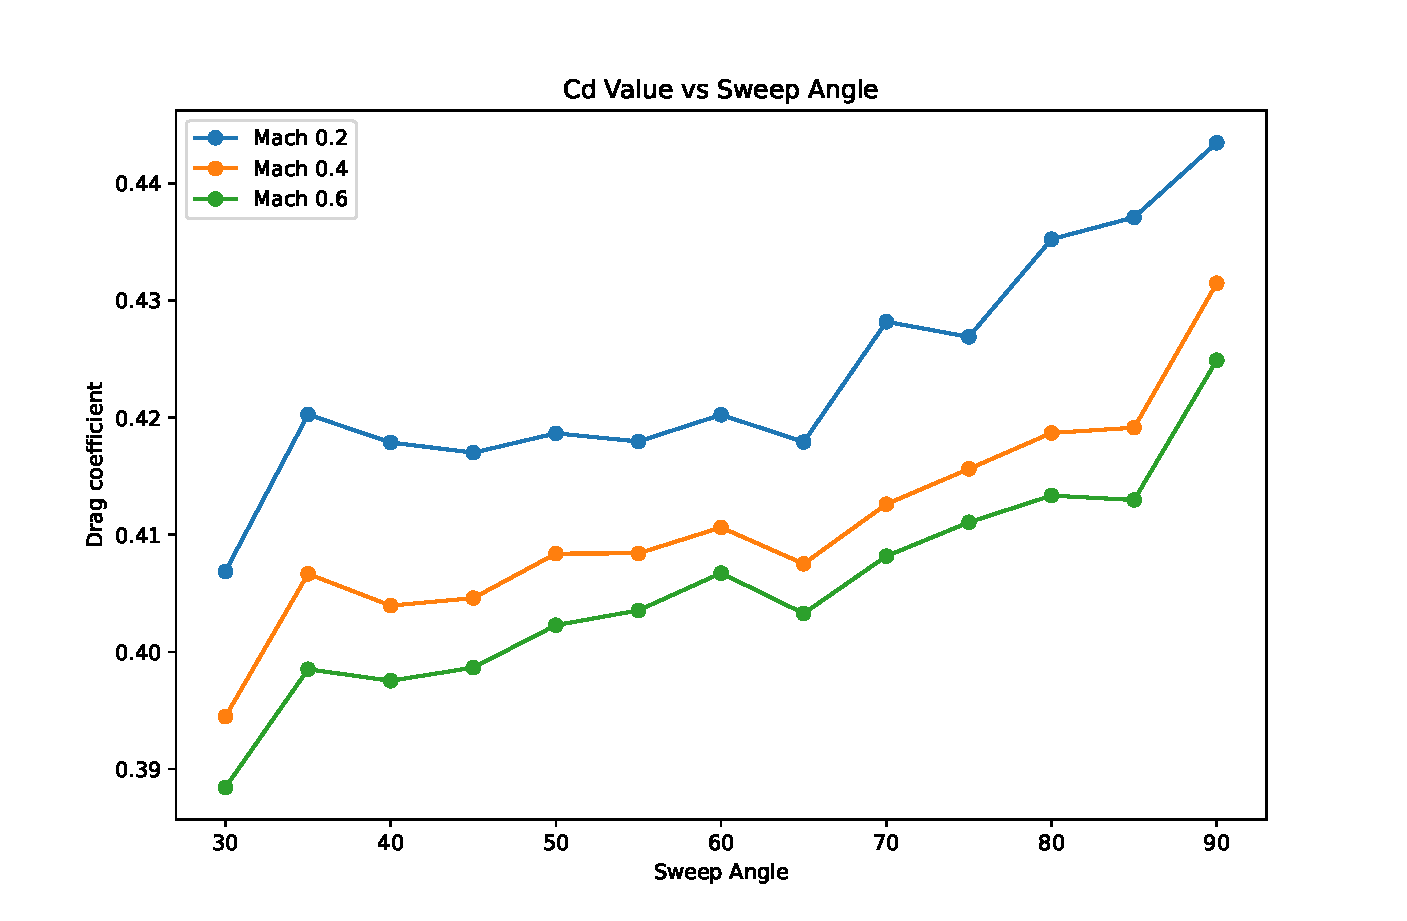
\includegraphics[width=0.8\textwidth]{../data/R6-Parametric-Fins/CDvsSweep.pdf}
    \caption{Drag coefficient vs Sweep Angle}
    \label{fig:CdVsSweep}
\end{figure}

\begin{figure}[H]
    \centering
    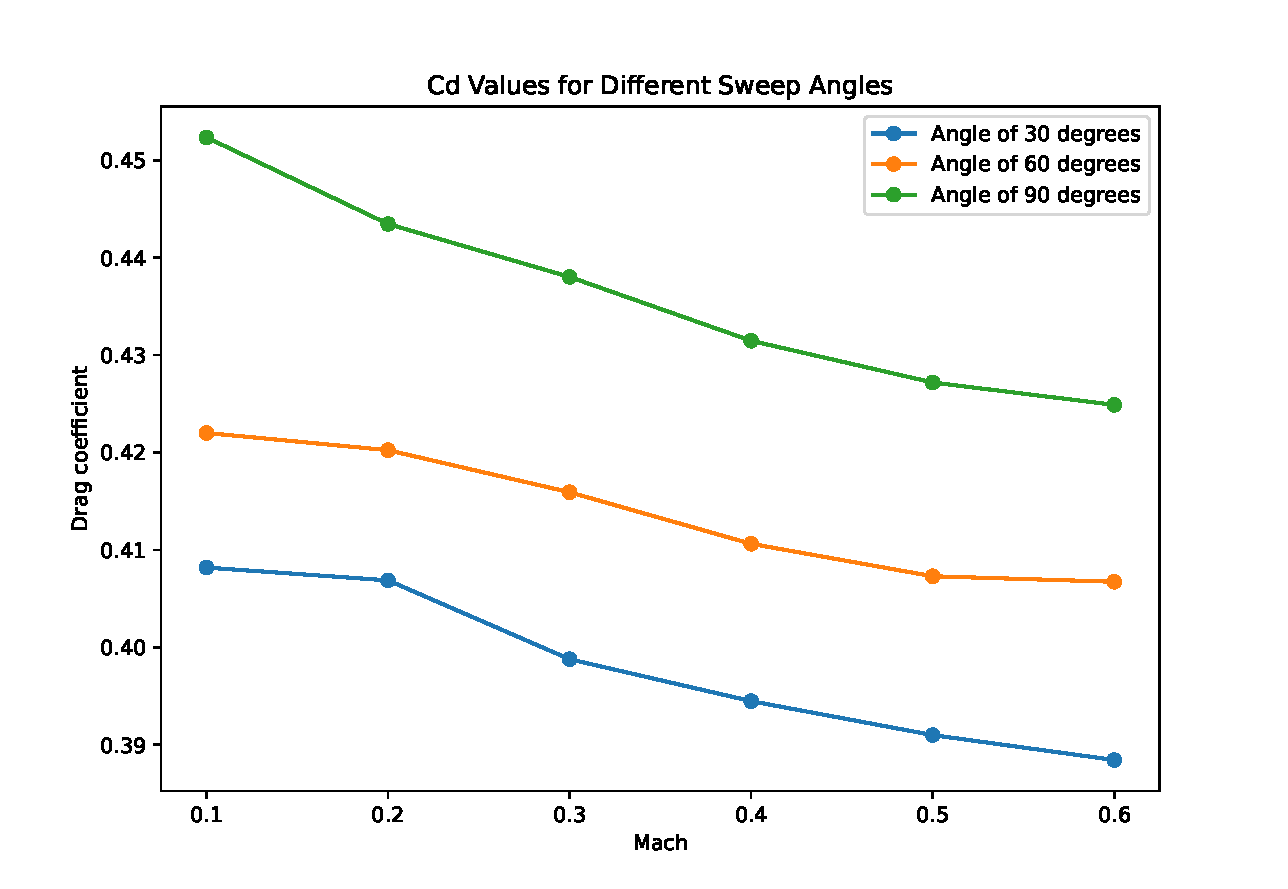
\includegraphics[width=0.8\textwidth]{../data/R6-Parametric-Fins/CDvsMach.pdf}
    \caption{Similarity of curves of drag coefficient vs Mach for different sweep angles}
\end{figure}

\section{Stability changes from OpenRocket}
\begin{figure}[H]
    \centering
    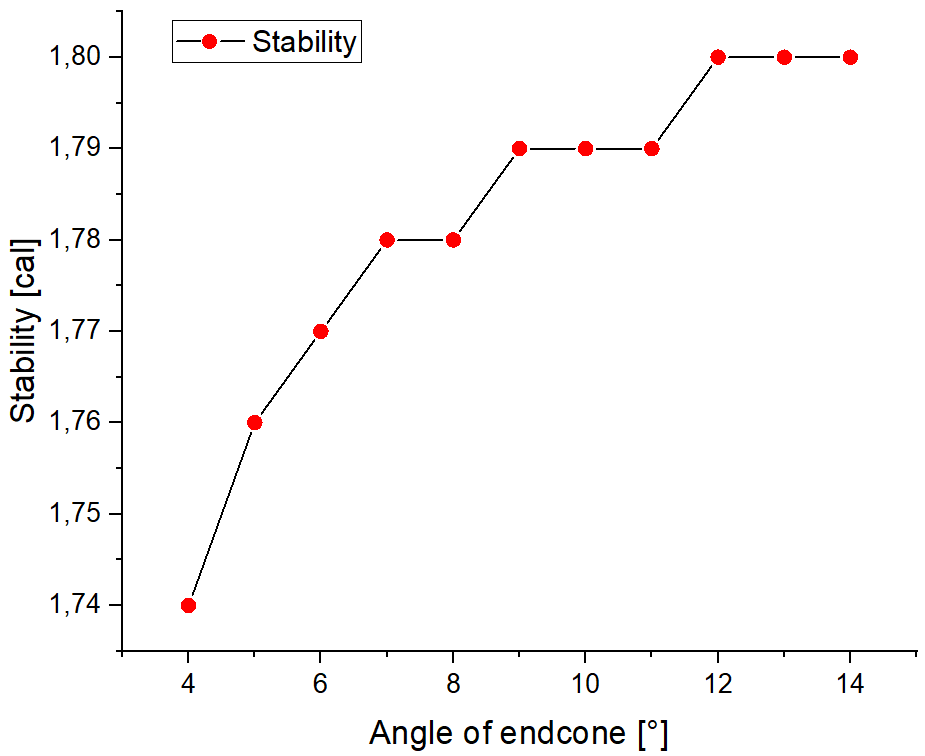
\includegraphics[width=0.7\textwidth]{../data/OR/EndconeStability.png}
    \caption{Stability graph vs Enconde Angle}
\end{figure}
\begin{figure}[H]
    \centering
    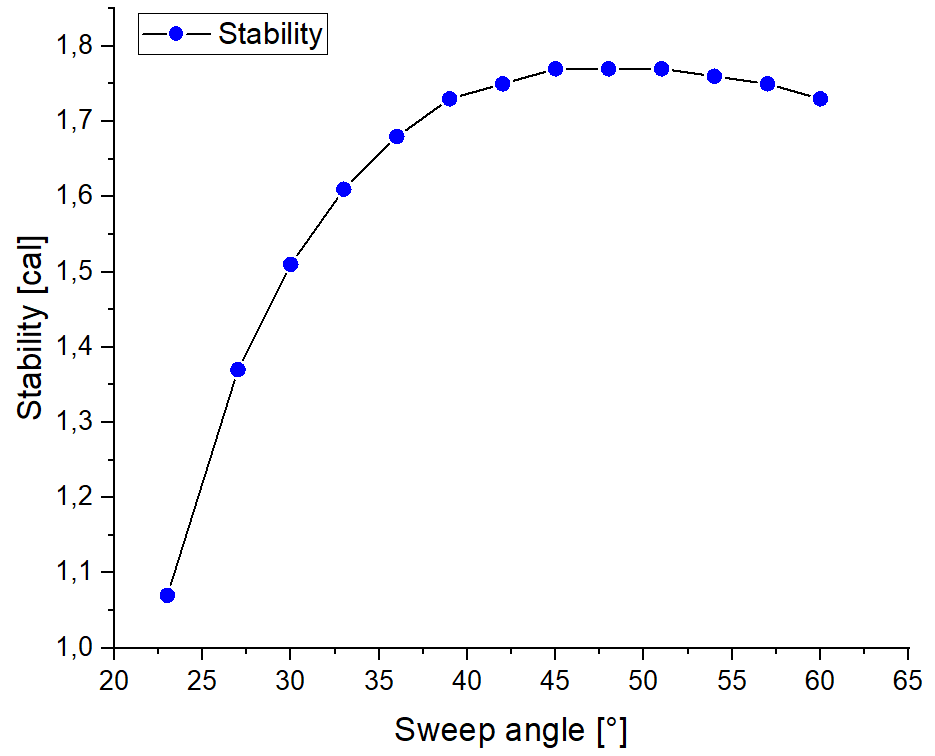
\includegraphics[width=0.7\textwidth]{../data/OR/FinStability.png}
    \caption{Stability graph vs Sweep Angle}
\end{figure}
\section{Summary}
In conclusion, it was found that the configuration with an endcone offers significantly better 
aerodynamic performance than the one without. Additionally, optimal sweep angle was found.
\subsection{Results of the preliminary research}

\begin{figure}[H]
    \centering
    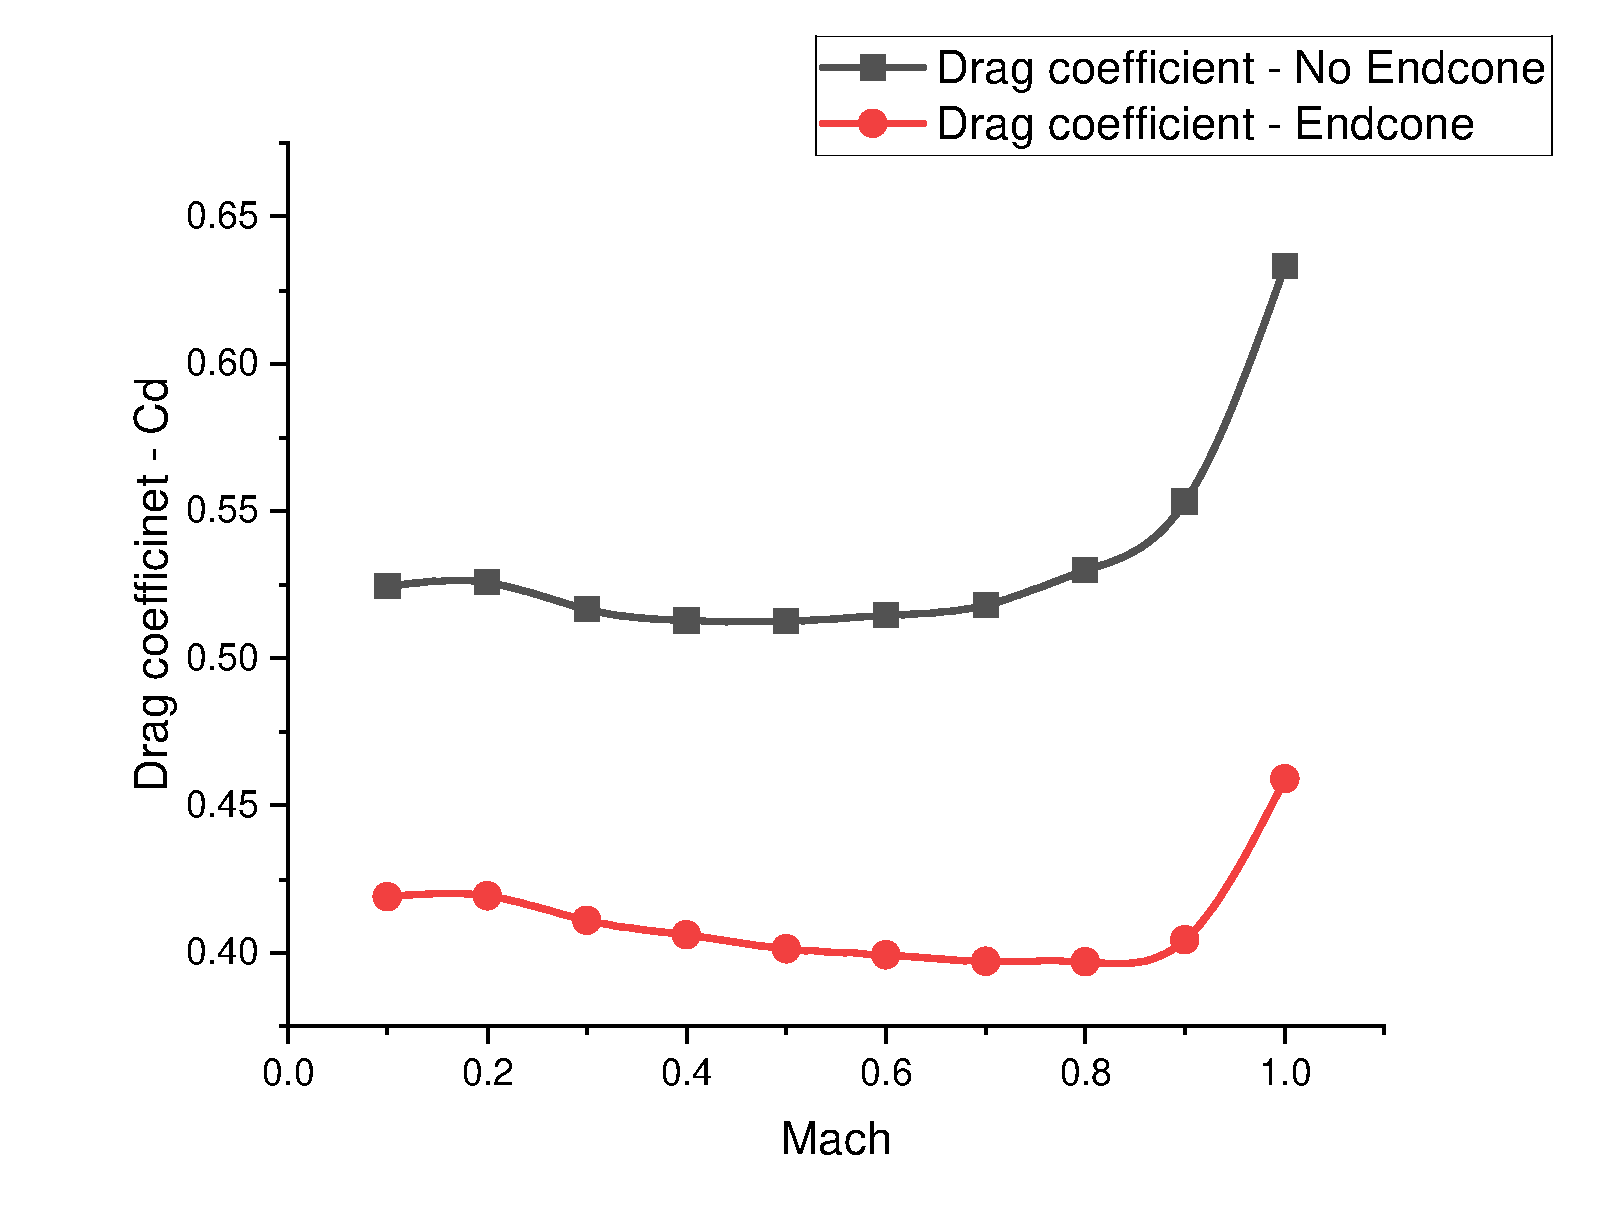
\includegraphics[width=\textwidth]{../data/DataAnalisysSolid/Solid-Studies-CD-Graph.pdf}
    \caption{CD graph of R6-Endcone and R6-NoEndcone models}
\end{figure}
Preliminary research indicates that the endcone model exhibits significantly lower drag coefficient
for 4.29 degrees endcone angle, while keeping similiar trends of change. Even more, for endcone model
the trans sonic spike starts later compared to no endcone model. This would be very beneficial for the
range of 0.6-0.9 Mach.  
\begin{table}[H]
    \centering
    \caption{Average values and differences}
    \resizebox{0.8\textwidth}{!}{%
    \begin{tabular}{|c|c|c|c|c|}
        \hline
        & R6 Endcone & R6 No Endcone & Difference & \% Difference \\
        \hline
        0.1 - 1.0 Mach & 0.411 & 0.534 & 0.123 & 29.8\%\\
        \hline
        0.1 - 0.6 Mach & 0.409 & 0.518 & 0.108 & 26.5\%\\
        \hline
    \end{tabular}%
    }
\end{table}
For a range of 0.1 to 0.6 Mach, the endcone model exhibited a 26\% lower drag coefficient in 
comparison to the no endcone model. This is a significant difference, indicating that the endcone
model is much more aerodynamically efficient.
\newpage

\subsection{Results of Endcone Optimalization}
The minimum of the average drag force function was found to be at 7 degrees. We can also 
observe a trend of the function, which is decreasing for the range of 3 to 7 degrees and increasing
for the range of 9 to 15 degrees.\\\\
Spike at 6 degree is worth mentioning, it may be true value at this point or just a result of
the simulation error. This would require further research to determine the validity of this spike, however 
it is not crucial for the optimalization of the rocket, since it is much higher than the minimum 
of the function and it's unlikely that noise of simulation was that high, especially that it can 
be seen at graphs of all example Cd vs Angle graphs for certain Mach number.
\begin{figure}[H]
    \centering
    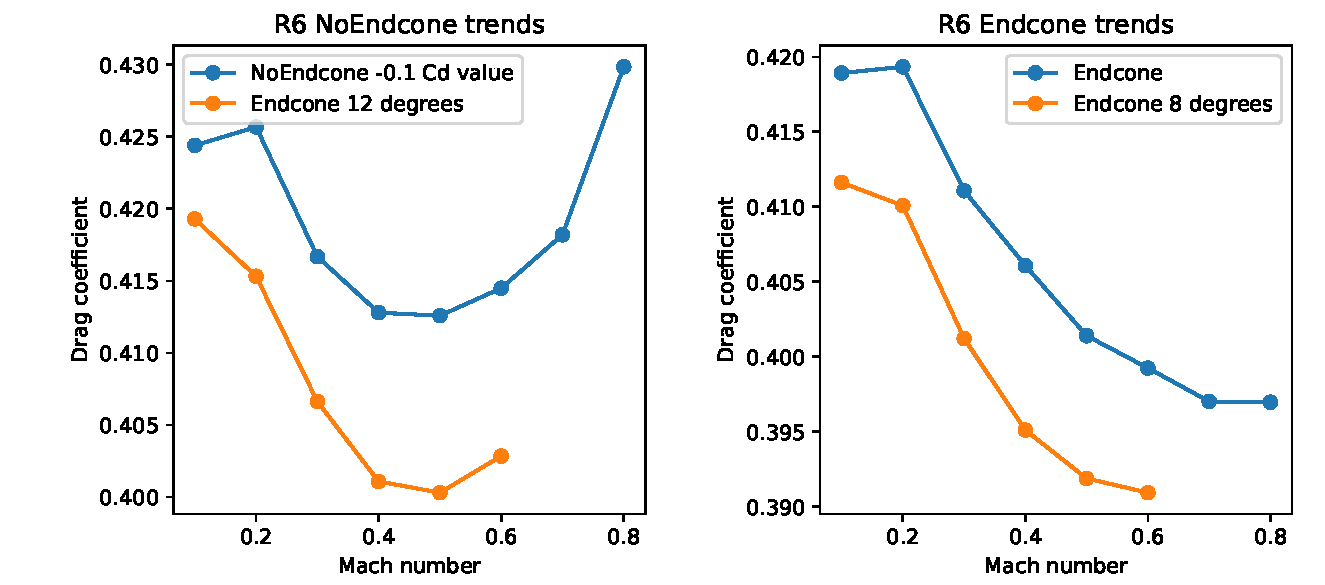
\includegraphics[width=0.9\textwidth]{../data/R6-Parametric-Endcone/comparisone2plots.pdf}
    \caption{Comparison of Drag coefficient vs Mach graph trends for different endcone angles}
\end{figure}
\noindent Key observation is that the transonic spike starts later for the endcone model with optimal
endcone angles, which
is very beneficial for the range of 0.6 to 0.9 Mach. This is an important finding from the
perspective of future rocket projects, where the rocket will be operating in this range of Mach.
For such rockets, optimal endconoe angle could generate significant savings in energy.\\\\
This observation could be already noticed in the preliminary research, where the Endcone model
exhibited decreasing trend of drag coefficient for the range of 0.6 to 0.8 Mach, while the NoEndcone
model exhibited a significant increase trend from 0.5 Mach forwards.

\subsection{Discussion of Fin Optimalization}
As shown in the Figure \ref{fig:ForceVsSweepAngle}, the minimum of the average drag force function is at 30 degrees. The function
is increasing for whole tested range, with relatively small local extremums at 35 and 65 degrees. This
means that the optimal sweep angle for the fins is 30 degrees. It could be also assumed that the
trend will continue to decrease for the range of 30 to 0 degrees, however too small sweep angle
would be impractical for the rocket, so it was not tested.\\\\

Figure \ref{fig:CdVsSweep} shows the same trend as the average drag force function, but 
also confirms the existence of characteristic local extremums at 35 and 65 degrees. This is a very
 important finding from the perspective of the optimalization of the rocket, since when desinginig 
the rocket, there was a prefered range of sweep angle. This study now clearly shows that when 
deling with the range of the sweep angle from 55 to 90 degrees, most aerodynamicly efficient
point likely to be close to 65 degrees.


\end{document}